\chapter{Background}
In this chapter, we provide the necessary theoretical and physiological background in cardiac electrophysiology and the application of PINNs in this context. We begin with an overview of the human heart's anatomy and the fundamental principles of cardiac electrophysiology, including the cellular mechanisms of excitability and the propagation of electrical signals through the heart tissue. We then dive into the mathematical modeling of cardiac electrophysiology, detailing the ionic models and the monodomain model classically used to describe the electrical activity of the heart. Following this, we introduce the concept of PINNs, explaining their architecture, the role of automatic differentiation, and how they are utilized to solve differential equations governing cardiac electrophysiology. 
\section{Cardiac Electrophysiology }
We begin with an in-depth exploration of the physiological and theoretical foundations of cardiac electrophysiology. The structure of the human heart is described first, highlighting the roles of the various chambers and the pathways of blood flow. Next, we examine the cellular mechanisms that enable cardiac muscle cells, or cardiomyocytes, to generate and propagate electrical signals, focusing on the concepts of membrane potential, depolarization, and repolarization. This discussion transitions into the mathematical representation of these processes through ionic models, particularly the Aliev-Panfilov model, which captures the dynamics of action potentials. Finally, we introduce the monodomain model, a volume-averaged approach to modeling the heart's electrical activity. This model simplifies computational complexity while maintaining accuracy in simulating the propagation of electrical waves through cardiac tissue. 
 
\subsection{The human heart}


The human cardiovascular system is powered by the heart, which acts as a pump to circulate blood throughout the body. The human heart is an amazing organ, pumping an incredible 7600 liters of blood each day without pause, a feat that no other muscle in the body can match. As illustrated in Figure \ref{fig:heart_illustration}, the heart is made up of four chambers: the right atrium (RA), the right ventricle (RV), the left atrium (LA), and the left ventricle (LV). The heart can be seen as two pumps that work in sequence, with the RA and RV carrying deoxygenated blood from the veins to the lungs through the pulmonary arteries. The blood is then oxygenated in the lungs before being sent through the pulmonary veins to the LA and then the LV. Finally, oxygenated blood is pumped out of the heart through the aorta~\cite{A.M.Katz}.

\begin{figure}[H]
    \centering
    \includesvg[width=0.6\linewidth]{Figs/Diagram_of_the_human_heart.svg}
    \caption{Diagram of the human heart with arrows indicating the direction of the blood-flow. Illustrated by Eric Pierce via Wikimedia Commons, licensed under CC BY-SA 3.0}
    \label{fig:heart_illustration}
\end{figure}

The heartbeat is generated by the collective contraction of cardiac muscle cells, known as cardiomyocytes. This process is managed by a complicated signal transmission system, where contractions are initiated by the sinoatrial (SA) node, forming what is known as a functional syncytium~\cite{2006Ctea}. The SA is located in the RA and produces electrical impulses that cause the atria to contract, thus pumping blood into the ventricles. The electrical impulses, transmitted through local activation of the cardiomyocytes, are then conducted to the atrioventricular node (AV), with a brief pause to allow the ventricles to fill with blood, then further on through the cardiac conduction system's His-Purkinje network to activate the ventricles to contract~\cite{HallJohnE2011GaHt}.

\subsection{The cell membrane and excitable tissue}

%The cells membrane
%The cell membrane is a cellular organelle that serves as a barrier between the inside and outside of the cell, referred to as the intracellular and extracellular domains. It encircles the cell and keeps the two domains separate. The cell membrane is composed of phospholipids, which have both hydrophobic and hydrophilic properties. When these molecules are in contact with water, they form a lipid bilayer, with the hydrophobic tails shielded from the water and the hydrophilic heads exposed in order to reduce the hydrophobic interaction. The lipids are not bound together, allowing them to move relative to each other and allowing other molecules to pass through. The interior of the membrane is nonpolar, so polar, electrically charged particles are not able to enter as this would cause significant hydrophobic interaction.

%Cardiomyocites & action potential
Cardiomyocytes (heart muscle cells) are excitable, which means that they can respond to electrical stimuli. At rest, these cells maintain ionic concentrations that differ from those of their surroundings. Because ions carry electrical charge, a potential difference arises between the inside and outside of the cell, known as the transmembrane potential (TP).
When electrical stimuli are applied to excitable cells, the TP increases. If the stimulus is strong enough, the cell's conductive properties change, leading to a flow of positive ions into the cell. This results in the TP increasing from a negative value to a positive value or close to zero, a process referred to as membrane depolarization. Heart cells stay in this depolarized state for a significant amount of time, typically a few hundred milliseconds, called the plateau phase. After depolarization, the potential returns to its resting value during a process called repolarization. The entire cycle consisting of depolarization followed by repolarization is termed a cardiac action potential (AP)~\cite{2006Ctea}.
\begin{figure}[H]
    \centering
    \includesvg[width=0.6\linewidth]{Figs/Ventricular_myocyte_ap.svg}
    \caption{Illustration of ventricular action potential with its five phases:  (0) \textit{depolarization}, (1) \textit{initial repolarization}, (2) \textit{plateau}, (3) \textit{repolarization}, (4) \textit{Resting potential}. Illustrated by Wikimedia Commons user Ksheka , licensed under CC BY-SA 3.0}
    \label{fig:AP}
\end{figure}

%The cell membrane as a capacitor


We now shift our focus from the physiological basis of overall cardiac function, excitability and conduction to a theoretical point of view, considering the mathematical modeling of excitable tissue. The electrical behavior of excitable cells can be represented as an electrical circuit composed of a combination of resistors and capacitors, with variable resistors acting as ion channels that enable ions to move in and out of the cell.
\begin{figure}[H]
  \centering
  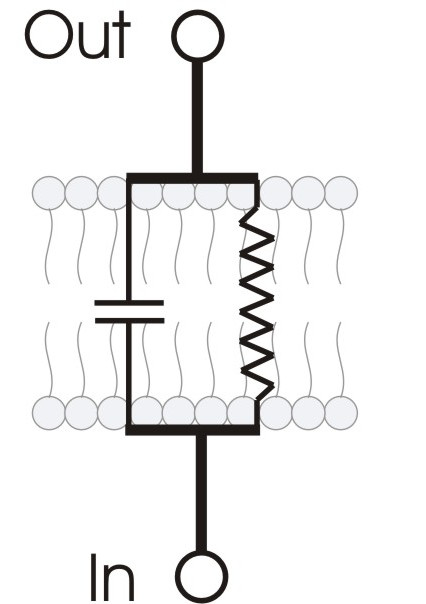
\includegraphics[width=0.3\textwidth]{Figs/RC_membrane_circuit.jpg}
  \caption{Resistor-capacitor circuit model of the cell membrane. Adaptation of illustration made by Wikipedia user Synaptidude, licensed under GNU Free Docummentation License}
  \label{fig: RC-membrane}
\end{figure}
In a capacitor, the charge is stored in two conductive plates separated by a dielectric and the ability of a capacitor to store charge is termed its capacitance. Since the cell membrane acts as an insulator with selective permeability to various ions, it can be viewed as a capacitor. The membrane capacitance, $C_m$, is defined as
\begin{equation}
    C_m = \frac{Q}{V},
    \label{eq:capacitance}
\end{equation}
where $Q$ is the charge across the cell membrane and $V$ is the electric potential needed to hold that charge.
Resistors represent the ion channels that allow the flow of ions across the membrane. The resistance of these channels, $R$, is inversely proportional to their conductance.

Kirchhoff's current law states that the net current flowing into a junction must be equal to the net current flowing out of the junction. In the context of the cell membrane, this can be written as
\begin{equation}
    I_{ion} + I_{cap}=0,
    \label{eq:KCL}
\end{equation}
where $I_{ion}$ is the net ionic current across the membrane and $I_{cap}$ is the capacitive current due to the charging and discharging of the membrane. Since current can be defined as $\frac{dQ}{dt}$, it follows that
\begin{equation}
    C_m\frac{dV}{dt} + I_{ions}=0.
    \label{eq:DE}
\end{equation}
This basic equation forms the basis for more complex models of excitable cells.







\subsection{The Aliev-Panfilov Ionic Model} 
In order to be able to represent the action potential in its entirety, we need an ionic model that accounts for both depolarization and repolarization. The Aliev-Panfilov model uses two state variables to do this:

\begin{equation}
I_{ion}=-kV(V-a)(V-1)-VW,
    \label{eq:AP_ionic}
\end{equation}

\begin{equation}
\label{eq:dwdt}
    \frac{dW}{d\tau}= (\epsilon + \frac{\mu_1W}{V+\mu_2})(-W-kV(V-b-1)),
\end{equation}
where $V$ is an adimensional variable that diffuses across neighboring cells, and $W$ is a non-diffusible variable, called a recovery variable which governs the restitution properties of the action potential.
%$v_n=100\frac{\mathrm{mV}}{\mathrm{AU}}$ and $\tau_n=12.9\frac{\mathrm{ms}}
$V$ is given in arbitrary units($\mathrm{AU}$) and relates to the transmembrane potential by $V=\frac{V_m-v_r}{v_n}$, where $v_r=-80\mathrm{mV}$ is the resting potential of the cardiac tissue and $v_n=100\mathrm{mV}\mathrm{AU^{-1}}$ is a normalization constant. Furthermore, time $\tau$ is measured in temporal units($\mathrm{TU}$) such that $t[\mathrm{ms}]=12.9\tau[\mathrm{TU}]$. The parameters $a$, $b$, $k$, $\mu_1$, $\mu_2$ and $\epsilon$ are generally selected based on empirical data to mimic the observed electrical signals \cite{EP-PINNs}.

\subsection{The Monodomain Model}
Up until now, we have focused on studying excitable tissue at the cellular level. However, it is not practical to model an organ as large as the heart by modeling each individual cell separately due to computational and other constraints. Hence, we move over to a volume averaging approach and consider the body as a volume conductor. The following derivations are based on \cite{Lines2002_bidomain}.

For a volume conductor, Farday's law states that \cite{griffiths2013introduction}

\begin{equation}
    \mathbf{\nabla} \times \mathbf{E}=-\frac{\partial \mathbf{B}}{\partial t},
    \label{eq:faraday}
\end{equation}

where $\mathbf{E}$ is the electric field and $\mathbf{B}$ is the magnetic field.
In the quasi-static approximation, the temporal variations of the magnetic field are negligible due to the relatively slow ion movements compared to the propagation of electromagnetic waves. This simplifies \eqref{eq:faraday} to 
\begin{equation}
    \nabla\cross\mathbf{E}=0,
\end{equation}
which states that the electric field has zero curl, and can thus be expressed as the gradient of a scalar potential $\phi$:

\begin{equation}
    \mathbf{E}=-\nabla \phi.
    \label{eq:scalar_potential}
\end{equation}
This relationship states that the electric field points in the direction of the steepest decrease in voltage, which entails that positively charged ions will move from high to low potential, and the opposite for negatively charged ions.

Since the velocity of charges can be ignored, the current density $\mathbf{J}$ is described by Ohm's law

\begin{equation}
    \mathbf{J}=\Sigma \mathbf{E },
    \label{eq:ohm}
\end{equation}
where $\Sigma$ is the conductivity tensor.

Combining \eqref{eq:ohm} and \eqref{eq:scalar_potential}, we can thus describe the current density in terms of the gradient of $\phi$ as  
\begin{equation}
    \mathbf{J}= -\Sigma \nabla \phi
    \label{eq:J_pot}
\end{equation}
The bidomain model considers the heart as composed of two overlapping continuous domains, namely the intracellular (subscripted $i$) and the extracellular domains (subscripted $e$) \cite{Tung_bidomain}. Let $\phi_i$ and $\phi_e$ be intracellular and extracellular potentials, respectively. The transmembrane potential, $V_m$, is then defined as the potential difference across the cell membrane such that

\begin{equation}
    V_m= \phi_i -\phi_e.
    \label{eq:Vm}
\end{equation}

From \eqref{eq:J_pot}, we can describe the current densities in the two domains as

\begin{equation}
    \mathbf{J_i}= -\Sigma_i \nabla \phi_i
    \label{eq:J_i}
\end{equation}
and
\begin{equation}
    \mathbf{J_e}= -\Sigma_e \nabla \phi_e.
    \label{eq:J_e}
\end{equation}

Any current leaving or entering one of the domains must do so through the membrane. Therefore, the change in current density in the intracellular and extracellular domain must be equal in magnitude with opposite sign \cite{Lines2002_bidomain}.

\begin{equation}
    \nabla \cdot \mathbf{J_i}=-\nabla \cdot \mathbf{J_e}=A_mI_m,
    \label{eq:transmembrane_current}
\end{equation}

where $I_m$ is the transmembrane current per unit area and $A_m$ is the surface to volume ratio of the cell membrane.

Combining \eqref{eq:J_e} and \eqref{eq:J_i} with \eqref{eq:transmembrane_current} yields our first bidomain equation

\begin{equation}
   \nabla \cdot (\Sigma_i \nabla \phi_i) = -\nabla \cdot ((\Sigma_i + \Sigma_e) \nabla \phi_e).
   \label{eq:bidomain_1}
\end{equation}

The transmembrane current can be described by a capacitive current and an ionic current

\begin{equation}
    I_m=C_m\frac{\partial V_m}{\partial t} + I_{ion}.
\end{equation}

Combining this with \eqref{eq:transmembrane_current} yields our final bidomain equation


\begin{equation}
\nabla \cdot (\Sigma_i \nabla V_m) + \nabla \cdot (\Sigma_i \nabla \phi_e) =A_m(C_m\frac{\partial V_m}{\partial t} + I_{ion})
\label{eq:bidomain2}
\end{equation}

The bidomain model, defined by \eqref{eq:bidomain_1} and \eqref{eq:bidomain2}, is computationally expensive. By assuming equal anisotropy rates, such that $\Sigma_e=\lambda \Sigma_i$, where $\lambda$ is a constant, the bidomain equations can be simpliflied to a single equation named the monodomain equation

\begin{equation}
\nabla \cdot (\Sigma_m \nabla V_m)=A_m(C_m\frac{\partial V_m}{\partial t} + I_{ion}),
\label{eq:monodomain}
\end{equation}
where it can be shown that the monodomain model is equivalent to the bidomain model if the conductivity tensor is given by the harmonic mean tensor $\Sigma_m$\cite{openCARP-sw}:
\begin{equation}
    \Sigma_m = (\Sigma_i\Sigma_e)(\Sigma_i + \Sigma_e)^{-1}.
\end{equation}

\begin{comment}

In this work, we will proceed with utilizing the monodomain model in combination with the Aliev-Panfilov ionic model given by \eqref{eq:AP_ionic} and \eqref{eq:dwdt}, which yields the following coupled equations with rescaled units
\begin{equation}
\label{eq:dvdt_AP}
    \frac{dV}{dt}=\nabla \cdot (\mathbf{\sigma}_m \nabla V) - kV(V-a)(V-1)-VW,
\end{equation}
and
\begin{equation}
\label{dwdt_AP}
    \frac{dW}{dt}= (\epsilon + \frac{\mu_1W}{V+\mu_2})(-W-kV(V-b-1)),
\end{equation}
\end{comment}

Additionally, in the monodomain model, it is reasonably assumed that no current is leaving the heart. This is imposed by no flux Neumann boundary conditions as

\begin{equation}
    \label{eq:no_flux}
    (\Sigma_m\nabla V_m)\cdot \vec{n}=0,
\end{equation}

where $\Vec{n}$ is the boundary normal.


\subsection{Monodomain combined with the Aliev-Panfilov Ionic Model}\label{mono_aliev}

Having introduced the components of the Aliev-Panfilov ionic model and the monodomain model, we now proceed to integrate these models together. In order to do this, we need to ensure dimensional consistency. Considering the ionic current $I_{ions}$ described in \eqref{eq:AP_ionic} in the Aliev-Panfilov model, we have
\begin{equation}
    I_{ion}=\left[\frac{\mathrm{AU}}{\mathrm{TU}}\right].
\end{equation}

Thus, it is necessary to determine a scaling coefficient, $\kappa$, to make sure that the units of the capacitive current and the diffusion term in \eqref{eq:monodomain} align with $I_{ion}$. Consequently, we then get

\begin{equation}
\kappa C_mA_m\frac{\partial V_m}{\partial t}=\left[\frac{\mathrm{AU}}{\mathrm{TU}}\right],
\label{eq:scale_cap}
\end{equation}
and
\begin{equation}
\kappa\nabla \cdot (\Sigma_m \nabla V_m)=\left[\frac{\mathrm{AU}}{\mathrm{TU}}\right].
\label{eq:scale_dif}
\end{equation}
We also have that

$$
V_m=v_nV-80\mathrm{mV} ~~\text{and}~~ t=\tau_n\tau,
$$

where $v_n=100\frac{\mathrm{mV}}{\mathrm{AU}}$ and $\tau_n=12.9\frac{\mathrm{ms}}{\mathrm{TU}}$ are normalization constants. We then get

\begin{equation}
\begin{aligned}
    \frac{\partial V_m}{\partial t}&= v_n\frac{\partial V}{\partial t}\\
    &=v_n\frac{\partial V}{\partial \tau}\frac{\partial \tau}{\partial t}\\
    &=\frac{v_n}{\tau_n}\frac{\partial V}{\partial \tau},
    \label{eq:scale_dVdt}
\end{aligned}
\end{equation}

and similarly

\begin{equation}
\begin{aligned}
    \nabla V_m &= \nabla (v_nV -80)\\
    &=v_n\nabla V.
    \end{aligned}
    \label{eq:scale_nablaV}
\end{equation}

Substitution of \eqref{eq:scale_dVdt} into \eqref{eq:scale_cap} gives
\begin{equation}
\kappa C_mA_m\frac{v_n}{\tau_n}\frac{\partial V}{\partial \tau}=\left[\frac{\mathrm{AU}}{\mathrm{TU}}\right],
\end{equation}

and since $\frac{\partial V}{\partial \tau}=\left[\frac{\mathrm{AU}}{\mathrm{TU}}\right]$, we must have

$$
\kappa = \frac{\tau_n}{v_nC_mA_m}.
$$

Similarly, we get

$$
\kappa\nabla \cdot (\Sigma_m v_n \nabla V)=\left[\frac{\mathrm{AU}}{\mathrm{TU}}\right],
$$

and we can thus define a diffusion tensor $D=\kappa v_n \Sigma_m$. In isotropic conditions, the conductivity is the same in all directions and the diffusion tensor can be reduced to a scalar value.

Finally, we obtain the following coupled equations with rescaled units
\begin{equation}
\label{eq:dvdt_AP}
    \frac{dV}{d\tau}=\nabla \cdot (D \nabla V) - kV(V-a)(V-1)-VW,
\end{equation}
and
\begin{equation}
\label{dwdt_AP}
    \frac{dW}{d\tau}= (\epsilon + \frac{\mu_1W}{V+\mu_2})(-W-kV(V-b-1)).
\end{equation}















\section{Physics Informed Neural Networks}
%
Having established the necessary physiological basis and theoretical background of the governing physics in this study, we now transition into the concept of PINNs. For a detailed description of neural networks the reader is referred to the work of Goodfellow et al. \cite{Goodfellow}. Our emphasis herein is on the framework of PINNs based on \cite{lu2021deepxde}.
A PINN is a type of neural network designed to solve both forward and inverse problems involving PDEs and ODEs. The general idea behind PINNs is that we can construct a loss function such that, when minimized, the
governing equations are satisfied by incorporating their
residuals into the loss function. In the approach first suggested by Raissi et al.\cite{RAISSI2019686}, a feed forward neural network (FFNN) is used to represent a target function. 

\subsection{Feed Forward Neural Network}
An FFNN is a computational model consisting of multiple layers of interconnected nodes. In these networks, as the name suggests, the information moves in only one direction, from input nodes, through hidden layers and to output nodes.

As described in \cite{lu2021deepxde}, let $\mathcal{N}(\theta,\mathbf{x}):\mathbb{R}^{n}\rightarrow \mathbb{R}^{m}$ be a neural network with inputs $\mathbf{x}\in \mathbb{R}^n$ and $m$ outputs, where $\theta$ are tunable parameters consisting of weights, $W^{\ell}\in \mathbb{R}^{N_{\ell}\times N_{\ell-1}}$, and biases $\mathbf{b}^{\ell}\in \mathbb{R}^{N_{\ell}}$ and $N_{\ell}$ is the number of nodes in layer $\ell \in [0,L]$. Regardless of the underlying architecture of the neural network, the resulting outputs will be linear transformations of the inputs. Consequently, introducing a non-linear activation function, $f$, is crucial in order to represent non-linear relationships. The neural network is thus a composite function defined as

\begin{align*}
\text{input layer:} \quad &\mathcal{N}^{0}(x) = x \in \mathbb{R}^{n}, \\
\text{hidden layers:} \quad &\mathcal{N}^{\ell}(x) = f(W^{\ell}\mathcal{N}^{\ell-1}(x) + b^{\ell}) \in \mathbb{R}^{N_{\ell}}, \\
\text{output layer:} \quad &\mathcal{N}^{L}(x) = W^{L}\mathcal{N}^{L-1}(x) + b^{L} \in \mathbb{R}^{m}, \\
\end{align*}

\subsection{Automatic differentiation}
Training a neural network involves determining the optimal parameters $\theta^*$. Central to this process is the backpropagation algorithm\cite{backprop}, which is a specific case of Automatic Differentiation (AD). The iterative procedure leverages the chain rule to update the network's weights and biases with the goal of minimizing a loss function. Considering the fact that the neural network represents a composite function, AD applies the chain rule repeatedly to compute the derivatives of the loss function with respect to the parameters $\theta$.
PINNs also  require computing the derivatives of the neural network outputs with respect to its inputs, which can be achieved by means of AD.
For simplicity, consider a neural with one input, $x$, one
hidden layer, and one output $y$. The forward propagation
then yields

\begin{equation*}
    \begin{aligned}
    \mathcal{N}^1&=W^1x + \mathbf{b}^1\\
    y&=W^2a^1 + \mathbf{b}^2,\quad \text{where } a^1=f(\mathcal{N}^1).
    \end{aligned}
\end{equation*}

Then by applying the chain rule, we can find the derivative of the output with respect to the input as follows

\begin{equation*}
\begin{aligned}
    \frac{\partial y}{\partial x}&=\frac{\partial y}{\partial a^1}\frac{\partial a^1}{\partial x}\\
    &=\frac{\partial y}{\partial a^1}\frac{\partial a^1}{\partial \mathcal{N}^1}\frac{\partial \mathcal{N}^1}{\partial x}\\
    &=W^2W^1f'(\mathcal{N}^1),
\end{aligned}
\end{equation*}

which demonstrates an important advantage of computing derivatives via automatic differentiation, primarily the fact that these derivatives no not depend on any discretization.
\subsection{PINN loss}

 We assign the first output to represent our estimate of $V$, and the second output to represent the estimate of the recovery variable $W$ such that

\begin{equation}
    \mathcal{N}^L=\begin{bmatrix}\Tilde{V}\\
    \Tilde{W}\\
    \end{bmatrix}.
\end{equation}
We can thus define residuals of Equations \eqref{eq:dvdt_AP} and \eqref{dwdt_AP} in terms of the neural network outputs and derivatives as

\begin{equation}
\label{eq:R_V}
R_V=-\frac{\partial \tilde{V}}{\partial \tau}+\nabla\cdot(D\nabla \tilde{V})-k \tilde{V}(\tilde{V}-a)(\tilde{V}-1)-\tilde{V} \tilde{W},
\end{equation}

and
\begin{equation}
\label{eq:R_W}
R_W=-\frac{\partial \tilde{W}}{\partial \tau}+\left(\epsilon+\frac{\mu_1 \tilde{W}}{\tilde{V}+\mu_2}\right)(-\tilde{W}-k \tilde{V}(\tilde{V}-b-1)).
\end{equation}
A hybdrid loss function $\mathcal{L}$ can then be defined as a combination of components which ensure both data fitting and consistency with the governing equations:

\begin{itemize}
    \item $\mathcal{L}_{\text{data}}$ ensures agreement with both voltage and recovery variable data for $N_d$ samples within the spatial domain $\Omega$ : \\
    \begin{equation}
    \mathcal{L}_{\text{data}} = \frac{1}{N_{d}} \sum_{i=1}^{N_{d}} \left(V(\vec{x}_i,t_i)-\Tilde{V}(\vec{x}_i,t_i)\right)^2+\frac{1}{N_{d}} \sum_{i=1}^{N_{d}} \left(W(\vec{x}_i,t_i)-\Tilde{W}(\vec{x}_i,t_i)\right)^2\quad \vec{x}_i\in \Omega
\end{equation}
    \item $\mathcal{L}_{PDE}$ and $\mathcal{L}_{ODE}$ account for the physical laws by evaluating the residual given by \eqref{eq:R_V} and \eqref{eq:R_W} evaluated at $N_c$ collocation points within $\Omega$ :
\begin{equation}
    \mathcal{L}_{PDE} = \frac{1}{N_{c}} \sum_{i=1}^{N_{c}} \left(R_{V}(\vec{x}_i, t_i)\right)^2\quad \vec{x}_i\in \Omega
\end{equation} 

\begin{equation}
    \mathcal{L}_{ODE} = \frac{1}{N_{c}} \sum_{i=1}^{N_{c}} \left(R_{W}(\vec{x}_i, t_i)\right)^2\quad \vec{x}_i\in \Omega
\end{equation}

    \item $\mathcal{L}_{\text{BC}}$ ensures no flux Neumann boundary conditions on $N_{BC}$ points sampled from the boundary $\partial \Omega$:
\begin{equation}
\mathcal{L}_{\text{BC}} = \frac{1}{N_{BC}} \sum_{i=1}^{N_{\text{BC}}} \left(\Vec{n} \cdot\left(D(\vec{x}_i)  \nabla\Tilde{V}(\vec{x}_i,t_i)\right)\right)^2\quad \vec{x}_i\in \partial \Omega:   
\end{equation}

\item and finally $\mathcal{L}_{\text{IC}}$ ensuring that the network's output $\tilde{V}$ at the initial time $t_0$ is close to the initial potential $V_0$ on $N_{ic}$ sampled data points
\begin{equation}
    \mathcal{L}_{\text{IC}} = \frac{1}{N_{\text{IC}}} \sum_{i=1}^{N_{\text{IC}}} \left(V(\vec{x}_i,t_0)-\Tilde{V}(\vec{x}_i,t_0)\right)^2\quad \vec{x} \in \Omega
\end{equation}
\end{itemize}

We then get

\begin{equation}
\centering
        \mathcal{L} =\lambda_{d}\mathcal{L}_{d a t a}+\lambda_{PDE}\mathcal{L}_{PDE}+\lambda_{ODE}\mathcal{L}_{ODE}
        +\lambda_{BC}\mathcal{L}_{V_{B C}}+\lambda_{IC}\mathcal{L}_{{I C}},  
\label{eq:pinn_loss}
\end{equation}
where \(\lambda_{d}\), \(\lambda_{PDE}\), \(\lambda_{ODE}\), \(\lambda_{BC}\), \(\lambda_{IC}\) are hyperparameters that weight the importance of each term in the loss function. Assigning these weights will be further discussed in the following chapter.






%Conventional approaches for solving partial differential equations (PDEs) that offer high accuracy and ease of implementation. However, their effectiveness is limited by the requirement to discretize a continuous domain. In recent years, there has been a growing interest in using neural networks as an alternative approach for solving PDEs. One of the main advantages is that neural networks offer a solution in the form of a function that can be evaluated continuously.\cite{Cybenko}

















